\documentclass[a4paper, 11pt]{article}
\usepackage{bookmark}
\usepackage[brazil]{babel}
\usepackage[utf8]{inputenc}
\usepackage{amsmath}
\usepackage{indentfirst}
\usepackage{graphicx,color}
\usepackage{multicol,lipsum}
\usepackage[top=3cm,bottom=2cm,left=3 cm,right=2cm]{geometry}
\usepackage{esvect}
\usepackage{setspace}
\usepackage{subcaption}
\usepackage{textcomp}
\usepackage{fontenc}[T1]
\usepackage{gensymb}
\usepackage{wasysym}
\setstretch{1.5}
\usepackage[table,xcdraw]{xcolor}
\usepackage{colortbl}
\usepackage{caption}
\usepackage{float}
%\usepackage[pdftex]{hyperref}
\bibliographystyle{acm}

\usepackage{listings}
\usepackage{xcolor}


\geometry{
    top=3cm,     % Margem superior
    bottom=2cm,  % Margem inferior
    left=2.5cm,  % Margem esquerda
    right=2.5cm  % Margem direita
}

\lstset{
    language=Python,
    basicstyle=\ttfamily\small,
    keywordstyle=\color{blue}\bfseries,
    stringstyle=\color{red},
    commentstyle=\color{gray},
    numbers=left,
    numberstyle=\tiny\color{gray},
    frame=single,
    breaklines=true,
    tabsize=1,
    showspaces=false,
    showstringspaces=false
}

\bibliographystyle{acm}

\begin{document}

\begin{titlepage}
	\begin{center}
	\begin{figure}[!ht]
	\centering
	
\includegraphics[width=6cm]{imgs/LNCC.png}
	\end{figure}
		LABORATÓRIO NACIONAL DE COMPUTAÇÃO CIENTÍFICA\\
		MESTRADO EM MODELAGEM COMPUTACIONAL\\ 
		\vspace{7cm}
		{\Large \textbf{Lista 2 - GA023 \\ Elementos de Processamento de Imagem}}
		\vspace{3cm}
	\end{center}
	
	\begin{flushright}
            Lorran de Araújo Durães Soares\\
	 \end{flushright}

	\begin{center}
		\vspace{\fill}
		 Petrópolis - RJ\\
         2024
	\end{center}
\end{titlepage}

\begin{titlepage}
	\begin{center}
        Lorran de Araújo Durães Soares \\
      \vspace{7cm}
      {\Large \textbf{Lista 2 - GA023 \\ Elementos de Processamento de Imagem}}
	\end{center}
\vspace{3cm}
	\begin{flushright}
   \begin{list}{}{
      \setlength{\leftmargin}{5cm}
      \setlength{\rightmargin}{0cm}
      \setlength{\labelwidth}{0pt}
      \setlength{\labelsep}{\leftmargin}}
      \begin{flushright}
          \item Trabalho apresentado  como  parte  dos  critérios 
de avaliação da disciplina GA023 - Elementos de Processamento de Imagem.
       \item Professor(a): Gilson Antonio Giraldi
      \end{flushright}
      
   \end{list}
	\end{flushright}

	\begin{center}
		\vspace{\fill}
		 Petrópolis - RJ\\
         2024
	\end{center}
\end{titlepage}

\tableofcontents
\newpage

\section{\textbf{Introdução}}

Este texto refere-se à lista realizada na disciplina GA023 Elementos de Processamento de Imagem, do curso de pós-graduação oferecido pelo Laboratório Nacional de Computação Científica (LNCC), sob a orientação do professor Gilson Antonio GIraldi. Neste documento, serão apresentadas as questões propostas pelo trabalho, seguidas de suas respectivas resoluções. O link para acessar o código referente a realização de cada uma das questões estará presente no final da descrição de cada questão aqui neste trabalho. Os exercícios foram realizados em Python usando bibliotecas como Numpy a Matplotlib.

\section{\textbf{Questão 1}}
\noindent Considere a distribuição normal bidimensional padrão (veja a página 32, referência [2]). 

(a) Usando versões discretas dessa função, construa um filtro passa-baixa.

(b) Agora, tome a derivada com respeito às variáveis x e y da distribuição normal bidimensional e repita o item anterior. Usando a transformada de Fourier de sequências e o respectivo teorema da convolução (teorema 3 do arquivo aula2.pdf), tente caracterizar o tipo de filtros obtidos.

(c) Aplique os filtros sobre uma imagem e analise os resultados.

\textbf{Resolução:}

Para a realização desta questão foi construído, através da biblioteca \texttt{Numpy}, um grid quadricular com dimensões $21 \times 21$, por meio do método \textit{meshgrid}. Então, foi definida a distribuição normal bidimensional com esse grid como domínio, na qual, de acordo com aula1.pdf, é dada pela equação:

\begin{equation}
    \mathtt{G}(x,y) = \dfrac{1}{\sqrt{2  \pi  \sigma^2}} \cdot \exp \left(\dfrac{-(x^2+y^2)}{2 \sigma ^2}\right)
    \label{norm_eq}
\end{equation}

De acordo com a aula1.pdf, temos que esse filtro é caracterizado por ser um passa baixa, como veremos mais adiante. A figura \ref{fig:norm_esp} mostra como ficou a visualização do filtro no domínio do espaço.

\begin{figure}[H]
    \centering 
    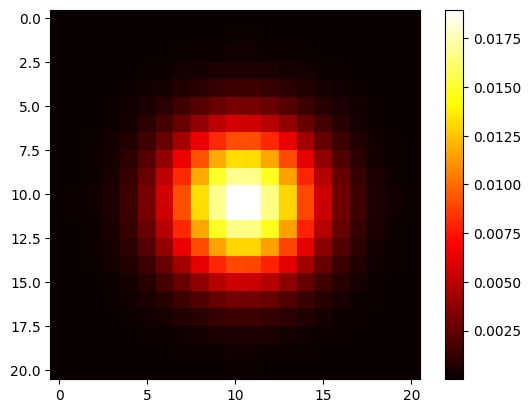
\includegraphics[width=0.7\textwidth]{imgs/norm_esp.png}
    \caption{Visualização do filtro Gaussiano no domínio do espaço}
    \label{fig:norm_esp} 
\end{figure}

Derivando a equação \ref{norm_eq} em relação a $x$ e a $y$, obtemos então as seguintes equações:

\begin{equation}
    \frac{\partial G}{\partial x}(x,y) = -\frac{x}{\sigma^3 \sqrt{2\pi}} \exp\left(-\frac{x^2 + y^2}{2\sigma^2}\right)
    \label{norm_eq_x}
\end{equation}

\begin{equation}
    \frac{\partial G}{\partial y}(x,y) = -\frac{y}{\sigma^3 \sqrt{2\pi}} \exp\left(-\frac{x^2 + y^2}{2\sigma^2}\right)
    \label{norm_eq_y}
\end{equation}

Usando o método \textit{fft} do \texttt{Numpy}, foram então transformados os filtros discretos determinados pelas equações \ref{norm_eq}, \ref{norm_eq_x} e \ref{norm_eq_y} para o domínio da frequência através da Transformada de Fourier. Logo, podemos plotar, usando a biblioteca \texttt{Matplotlib}, uma visualização de cada um dos filtros no domínio da frequência, obtendo as imagens da figura \ref{fig:fil_freq}.

\begin{figure}[H]
    \centering 
    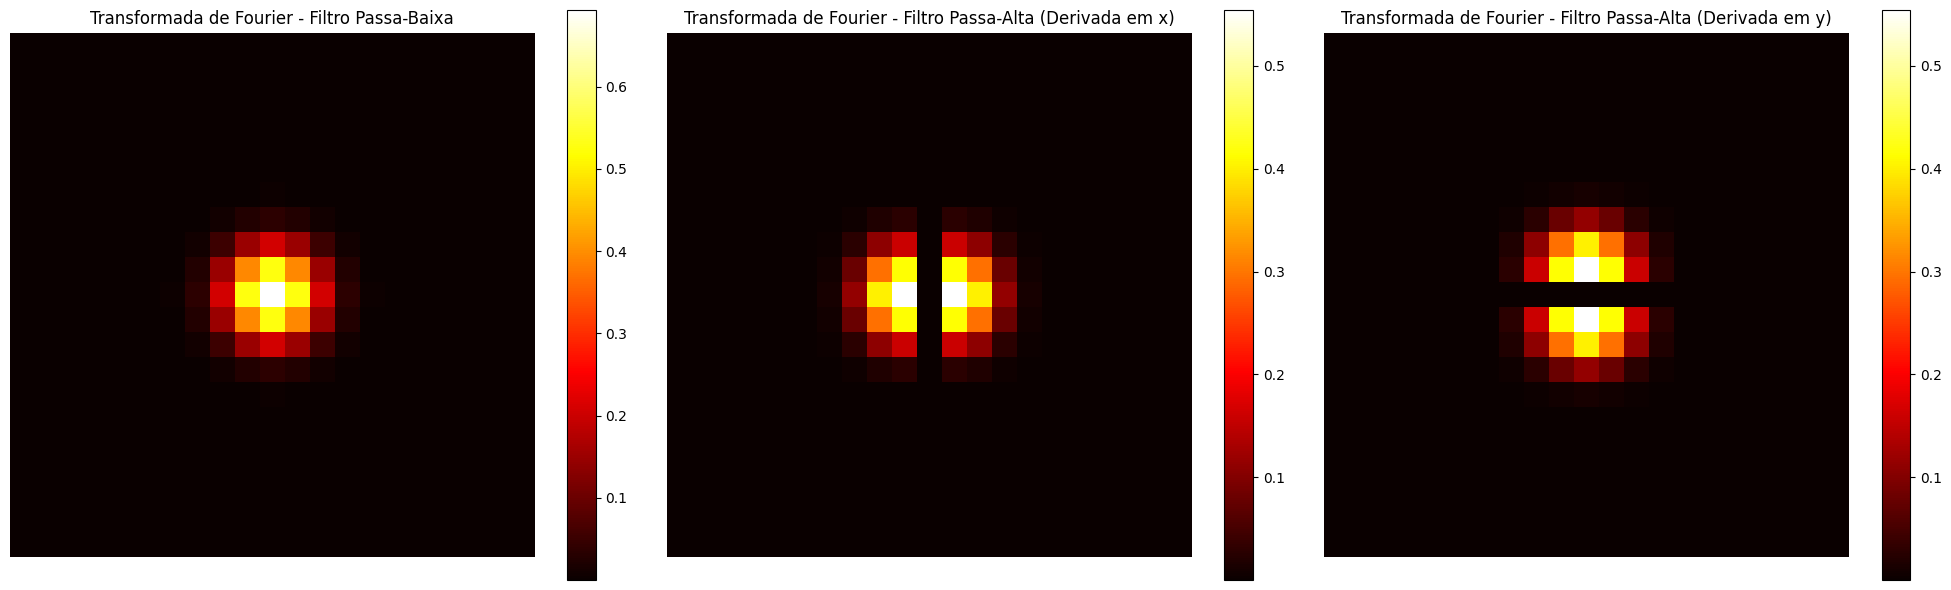
\includegraphics[width=1\textwidth]{imgs/filt_four.png}
    \caption{Visualização de cada filtro no domínio da frequência}
    \label{fig:fil_freq} 
\end{figure}

Sabendo que, segundo o teorema do convolução, teremos que a multiplicação direta do filtro com a transformada da imagem é equivalente a realização da convolução no domínio, podemos convluir que a primeira imagem se trata de um filtro passa baixa, pois as principais intensidades estão no centro da imagem, que se trata dos menores valores da frequência, enquanto as outras duas imagens demonstra que os filtros se tratam de band pass filtros, pois frequências proximas de 0 no eixo x e no eixo y vão ser anuladas pelos filtros gaussianos derivados parcialmente em relação a x e a y respectivamente.

Utilizando a biblioteca \texttt{Skimage} com as classes \textit{io} e \textit{color}, foi carregado uma imagem e convertida para tom de cinza. Usando o método \textit{convolve} da biblioteca \texttt{Scipy}, aplicamos os filtros a esta imagem, onde a biblioteca detecta automaticamente a complexidade do cálculo para decidir entre aplicar a convolução normalmente no domínio do tempo ou usar o teorema da convolução para aplicar no domínio da frequência e posteriormente voltar para o domínio do espaço. Ao terminar esses passos, foi então obtido o seguinte resultado presente na figura \ref{fig:ney}, que mostra a imagem original seguida das aplicações de cada filtro.

\begin{figure}[H]
    \centering 
    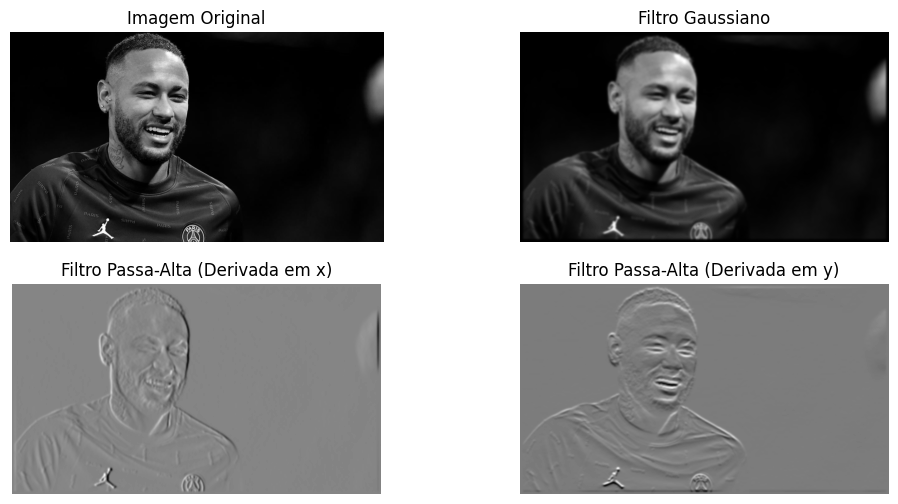
\includegraphics[width=1\textwidth]{imgs/ney.png}
    \caption{Visualização da aplicação dos filtros em uma imagem}
    \label{fig:ney} 
\end{figure}

Como podemos observar, os resultados foram condizentes com a classe do filtro, tendo o filtro passa baixa realizado uma suavização na imagem, enquanto nos filtros band pass houve detecção das frequências mais atenuantes geralmente presentes nas bordas dos elementos da imagem. Interessante observar que pelo derivado em relação a x, houve uma detecção das bordas no sentido do eixo x, e no eixo em relação ao eixo y.

% ===========================================================================================
% ===========================================================================================
% ===========================================================================================
% ===========================================================================================
% ===========================================================================================
% ===========================================================================================
% ===========================================================================================
% ===========================================================================================
% ===========================================================================================

\section{\textbf{Questão 2}}
\noindent \textit{Estude a teoria do PCA para problemas de pequeno tamanho de amostra, onde o número de dados é menor do que a dimensão do espaço de dados. Escolha um banco de dados de imagens, converta as imagens para escala de cinza e aplique a teoria de "PCA para problemas de pequeno tamanho de amostra" para redução de dimensionalidade.}

\begin{enumerate}
    \item[(a)] \textit{Se $\bar{x}$ é a média amostral (centroide do conjunto de dados) e $p_1$ é o componente principal, visualize o resultado da expressão:}
    \[
    x = \bar{x} + \alpha p_1,
    \]
    \textit{onde $\alpha \in \{-\beta \lambda_1, 0, \beta \lambda_1\}$ com $\lambda_1$ sendo o autovalor associado a $p_1$ e $\beta$ um fator escalar.}
    
    \item[(b)] \textit{Estude o espectro da matriz $X^T X$ para realizar a redução de dimensionalidade. Visualize algumas imagens no espaço de dimensão reduzida.}
    
    \item[(c)] \textit{Construa um gerador de imagens usando os $d$ componentes principais escolhidos no item (b).}
\end{enumerate}

\textbf{Resolução:}

Para realizar a redução de dimensionalidade usando Análise de Componentes Principais (PCA) em um conjunto de dados onde o número de amostras é inferior à dimensão do espaço dos dados, foi escolhida a base de imagens 'frontalimages\_spatiallynormalized' da FEI Face Database \cite{FEI}. Esta base é composta por 400 imagens faciais frontais, já em escala de cinza e normalizadas, de homens e mulheres, sérios e sorridentes, com resolução de $260 \times 360$ pixels. Todos os plots de imagens e gráficos foram realizados através da biblioteca \texttt{matplotlib} do Numpy. Para o carregamento dessas imagens, obtidas em \cite{FEI}, foram utilizadas as bibliotecas \texttt{OS} e \texttt{PIL}, que também realizaram a conversão das imagens para arrays numpy, o formato desejado para os cálculos subsequentes. A imagem \ref{fig:FEI} mostra alguns exemplos de imagens presentes nesse banco de imagens.

\begin{figure}[H]
    \centering 
    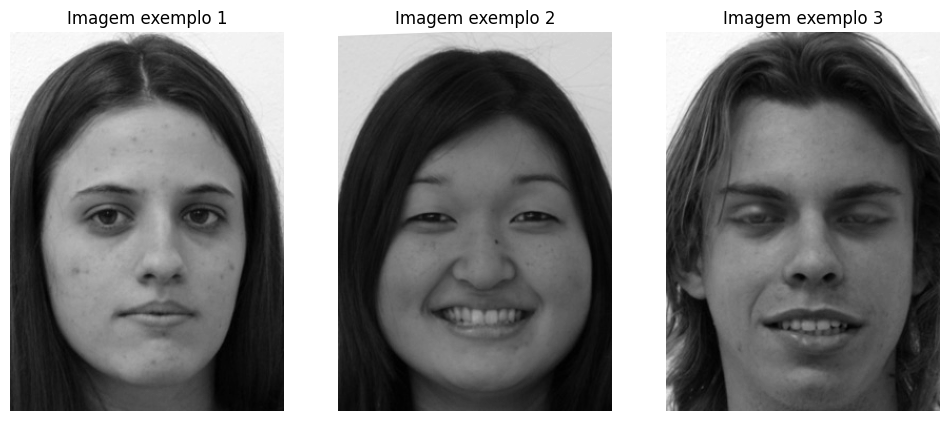
\includegraphics[width=0.8\textwidth]{imgs/FEI.png}
    \caption{Imagens geradas para o item (a)}
    \label{fig:FEI} % cria um rótulo para referência no texto
\end{figure}

Como este é um problema com poucas amostras em relação à dimensionalidade dos dados, para o cálculo da matriz $P_{PCA}$, com o objetivo de minimizar a perda de informação das imagens ao reduzir sua dimensionalidade, seguimos os passos descritos em Miranda. Aqui, $X$ representa a matriz de dados já vetorizada: 

\begin{enumerate}
    \item Calculo da matriz $\tilde{X}$ de dados centralizados pela expressão \[\tilde{X} = \begin{bmatrix}
    \tilde{x}_1^T \\
    \tilde{x}_2^T \\
    \vdots \\
    \tilde{x}_N^T
    \end{bmatrix}
    \in {R}^{N \times n},\]
    onde N é o número de amostras e n é a dimensão do espaço de dados (neste caso, $360 \cdot 260=93600$) e cada $\tilde{x}_i$ é centralizado da forma $\tilde{x}_i=x-\bar{x}$, onde $\bar{x}$ é a média dos dados.
    \item Resolução do problema de autovalores e autovetores para a matriz $\dfrac{1}{N} \tilde{X} \tilde{X}^T \in {R}^{N \times N}$:
    \[
    \ \dfrac{1}{N}\tilde{X} \tilde{X}^T v_i = \lambda_i v_i,
    \]
    \item Calculo dos vetores $\omega_i = \tilde{X}^T v_i, \quad i = 1, 2, \dots, N.$
    \item Normalização dos vetores $\omega_i$ para obter os autovetores da matriz de covariância $S = \dfrac{1}{N} \tilde{X}^T \tilde{X}$:
    \[
    a_i = \frac{\omega_i}{\|\omega_i\|} = \frac{\tilde{X}^T v_i}{\|\tilde{X}^T v_i\|}.
    \]
\end{enumerate}

Os autovetores obtidos ao final desse processo, ordenados em ordem decrescente em relação aos respectivos autovalores, são as colunas da matriz $P_{PCA}$ que queríamos. 

O cálculo dos autovetores e autovalores da matriz foi realizada através da função \texttt{np.linalg} e a multiplicação de matrizes foi calculada por meio da função \texttt{np.dot}, ambas presentes na biblioteca científica \texttt{Numpy}.

Para o item a, o resultado da expressão $\mathbf{x} = \bar{\mathbf{x}} + \alpha \mathbf{p}_1$, com $\alpha \in \{-\beta\sqrt{\lambda_1}, 0, \beta\sqrt{\lambda_1}\}$, com $\beta=0.8$, resultou nas imagens presentes na figura , onde $\lambda_1$ é o autovalor correspondente à componente principal $\mathbf{p_1}$. A legenda coeficiente 1 se trata do valor $-\beta\sqrt{\lambda_1}$, o coeficiente 2 é 0 e o coeficiente 3 é $\beta\sqrt{\lambda_1}$. As imagens demonstraram que a componente principal ficou mais responsável pelo fundo da imagem, que era um fator bem comum a todas as fotos.

% \begin{figure} [H]
%     \centering 
%     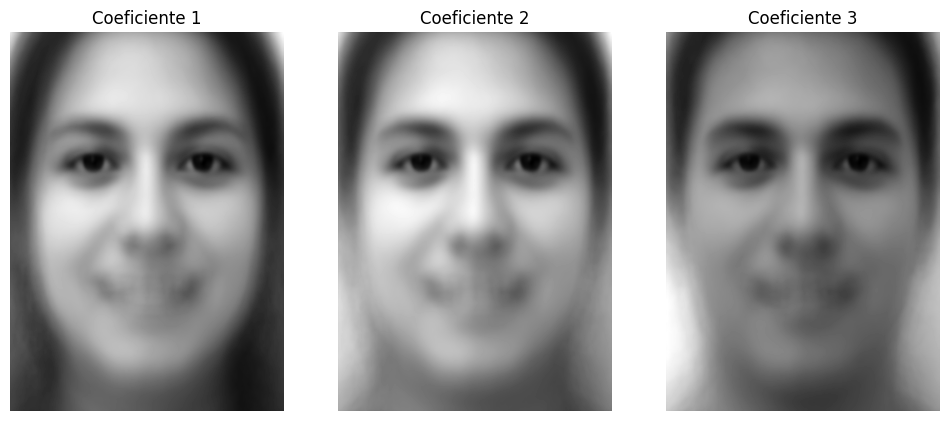
\includegraphics[width=0.8\textwidth]{imgs/a.png}
%     \caption{Imagens geradas para o item (a)}
%     \label{fig:a} % cria um rótulo para referência no texto
% \end{figure}

Para o item (b), ao calcular os autovalores da matriz $S = \dfrac{1}{N} \tilde{X}^T \tilde{X}$ e os ordenar em ordem descrescente, foi plotado o gráfico da variância explicada individual e acumulada dos autovalores, com o objetivo de analisar a contribuição de cada um na representação do conjunto de dados e identificar as principais componentes. A partir do gráfico , foi então decidido aplicar a redução para as 150 primeiras componentes , foi decidido aplicar a redução para as 150 primeiras componentes, pois estas já representavam mais de 90\% da energia total dos autovalores.

Foi então aplicado o truncamento multiplicando a matriz $P_{PCA}$ por $I_{150}$, onde I tem dimensão $400\times 400$, que é o tamanho das colunas da matriz $P_{PCA}$, mas tem até os primeiros 150 números da diagonal preenchido por 1, e todo o resto por 0. Para visualizar então como ficaram as imagens após essa redução, foi realizado o cálculo $X \cdot P_{PCA} \cdot P_{PCA}^T$, obtendo então as imagens presentes na  com a comparação com suas originais. Nas imagens, é notada a redução de qualidade e nitidez em relação à imagem original, mas de forma que as faces ainda mantiveram seus traços e podem ser reconhecidas.

% \begin{figure} [h]
%     \centering 
%     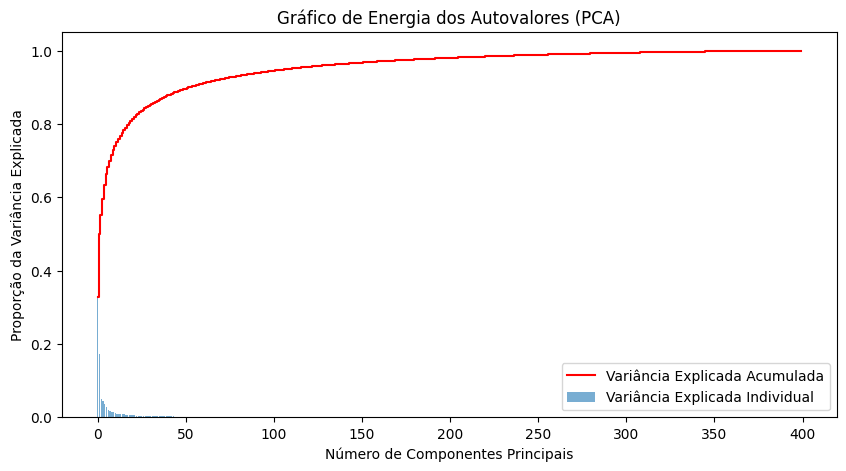
\includegraphics[width=0.8\textwidth]{imgs/var.png}
%     \caption{Gráfico de energia dos autovalores}
%     \label{fig:var} % cria um rótulo para referência no texto
% \end{figure}

% \begin{figure} [H]
%     \centering 
%     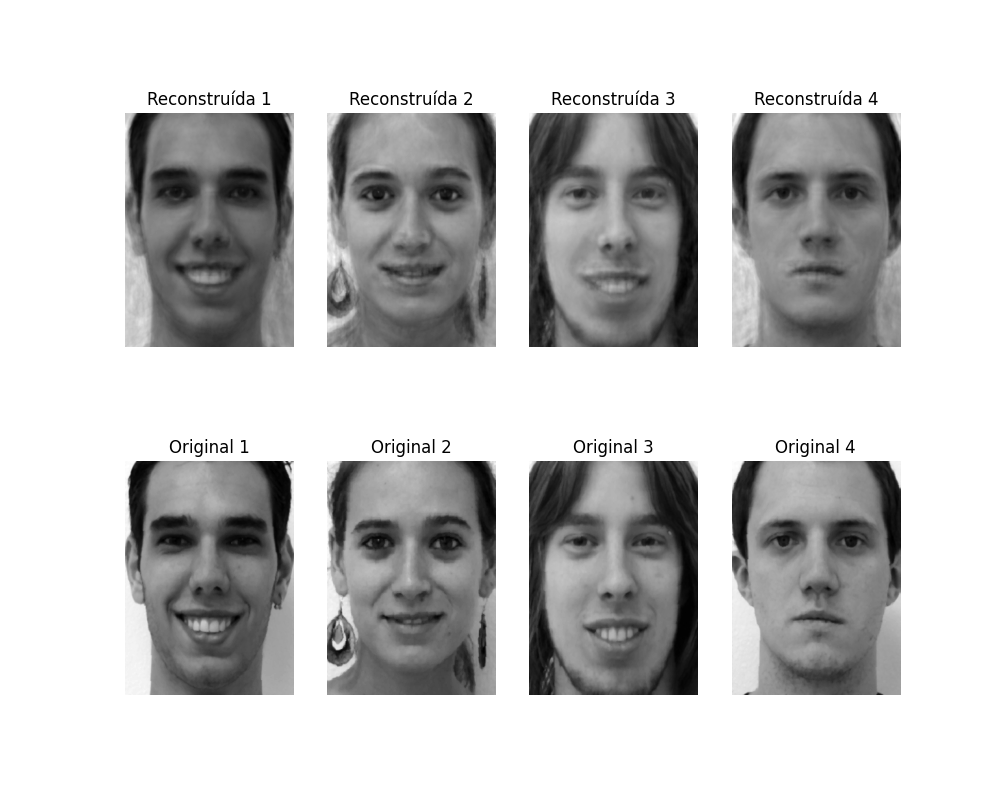
\includegraphics[width=1.0\textwidth]{imgs/comparacao_imagens.png}
%     \caption{Comparação reconstruída e original}
%     \label{fig:com} % cria um rótulo para referência no texto
% \end{figure}
Para o item (c), na construção do gerador de imagens, foi realizada a operação de maneira analoga ao item (a), só que agora, ao invés de usar apenas a primeira componente principal, foi considerado as 150 primeiras componentes principais. Para a seleção dos coeficientes $\beta$, através da biblioteca \texttt{numpy}, foi realizado o sorteio do número entre 0 e 1, com o uso de uma distribuição de probabilidade uniforme disponibilizada pela biblioteca denominada \texttt{np.random.uniform} , resultando, por exemplo, nas quatro imagens de novas faces, dada em . Ao realizar várias gerações, observou se faces com características bem diferentes, como lábios, sombrancelha e narizes. Em um dos testes realizados, no qual a imagem não consta aqui nestre trabalho, chegou a ser gerada uma pessoa de óculos e outras sem.

% \begin{figure} [H]
%     \centering 
%     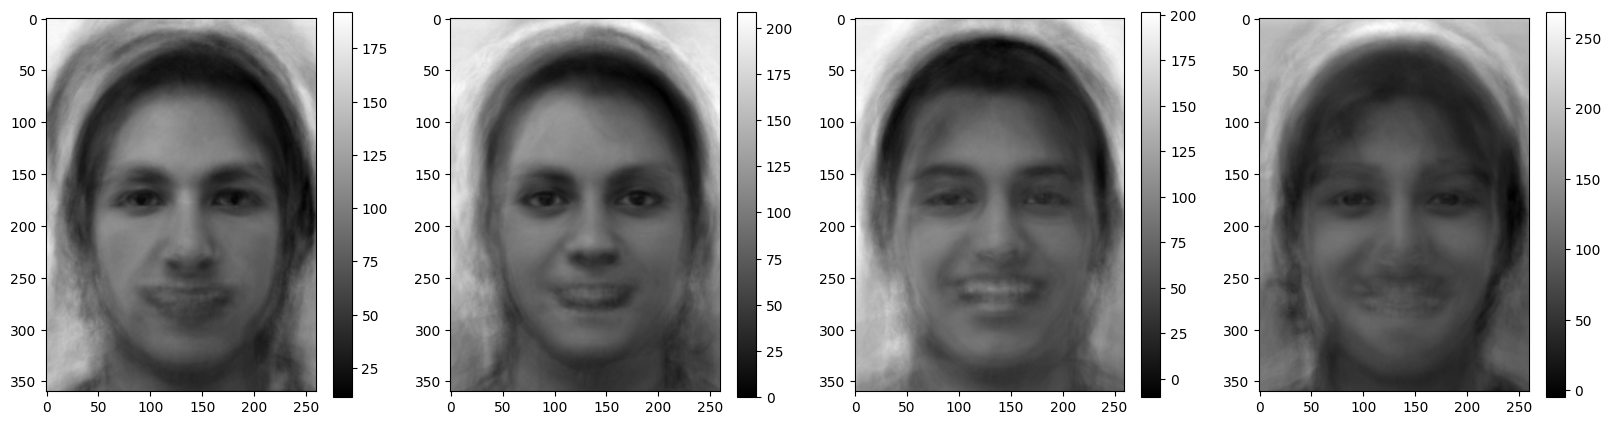
\includegraphics[width=0.7\textwidth]{imgs/gerador.png}
%     \caption{Imagem gerada pelas 150 primeiras componentes}
%     \label{fig:ger} % cria um rótulo para referência no texto
% \end{figure}

O código referente à realização do exercício descrito acima está disponível online na plataforma github. \href{https://github.com/lorran-araujo/LNCC/blob/main/disciplinas/redes-neurais/codes/lista2/exercicio3.ipynb}{Clique aqui para ver o código}.

% ========================================================================================

\bibliography{Bibliografia} 

\end{document}

